\documentclass[xcolor=dvipsnames]{beamer}
\usecolortheme[named=Green]{structure}
\usetheme{Boadilla}
\begin{document}
\author{Matthew Via and Victoria Chwalowski}
\title{Patrick Stewart}
\date{\today}
\theoremstyle{definition}
\newtheorem{fct}{Fact}
\theoremstyle{plain}
\newtheorem{qct}{Quote}
\begin{frame}{}
  \begin{columns}
    \begin{column}{0.5\textwidth}
      \titlepage
    \end{column}
    \begin{column}{0.5\textwidth}
      \begin{center}
        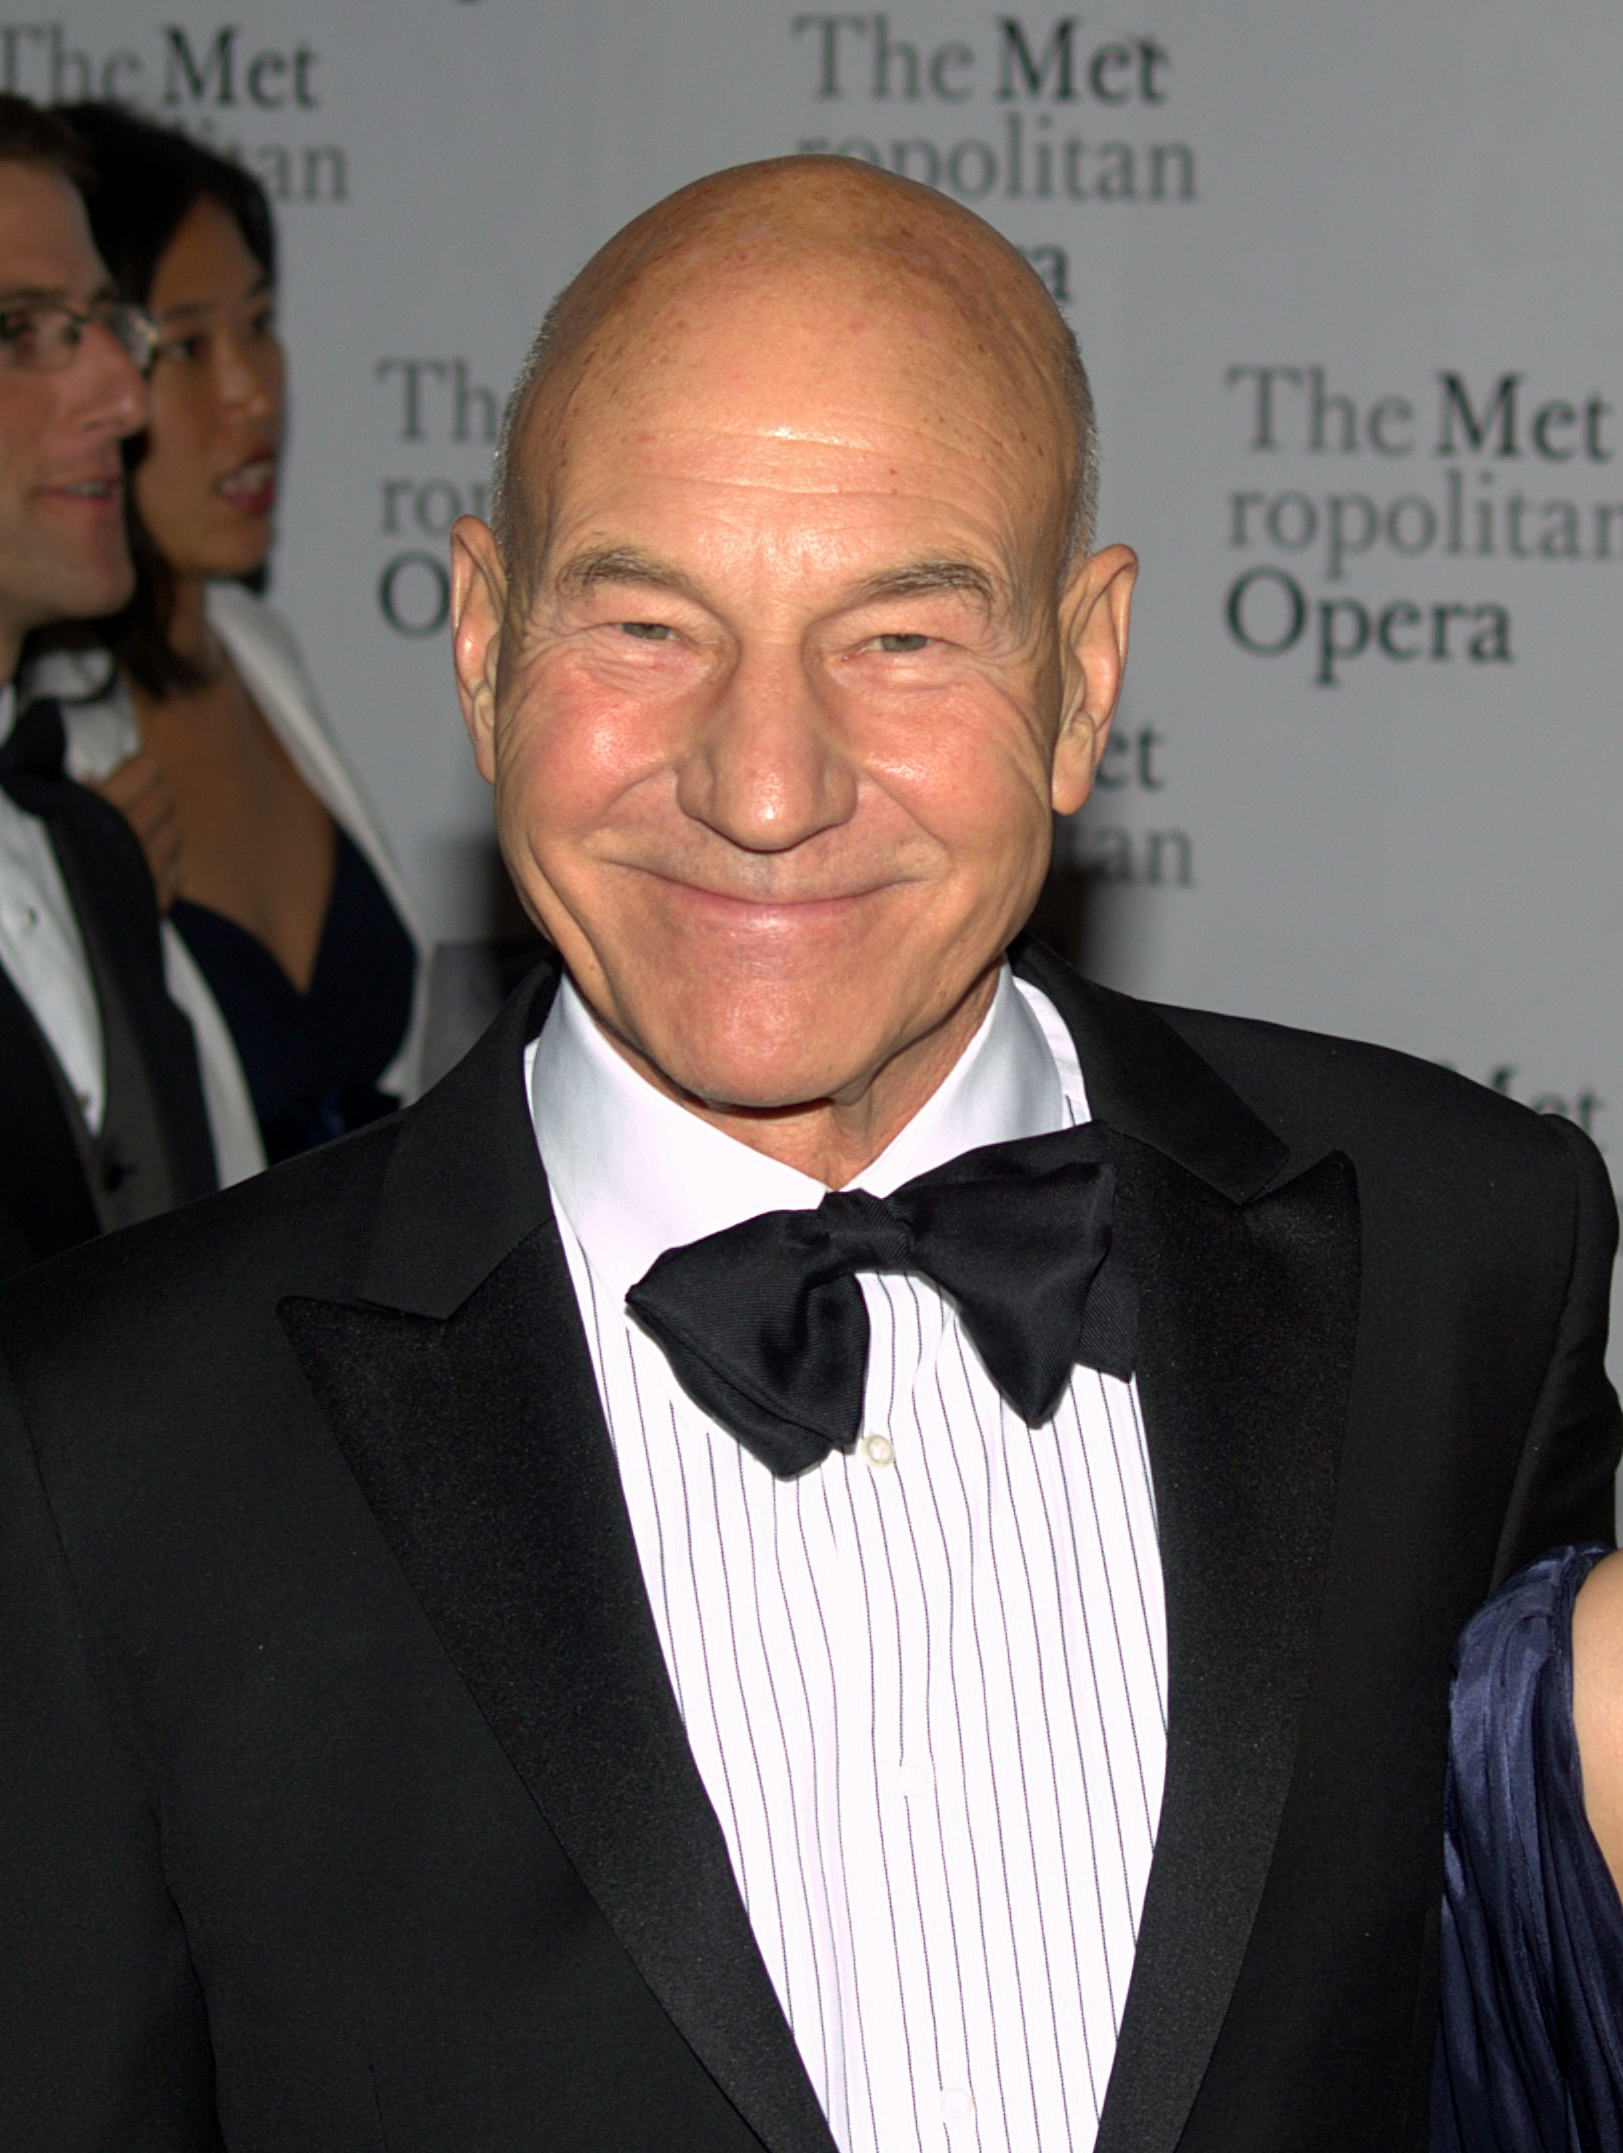
\includegraphics[width=0.8\textwidth]{smile.jpg}
      \end{center}
    \end{column}
  \end{columns}
\end{frame}

\begin{frame}{Early life}
  \begin{fct}
    Sir Patrick Stewart was born on 13 July 1940.
  \end{fct}
  \begin{itemize}
    \item Born to Gladys and Alfred Stewart
    \begin{itemize}
      \item Mother worked with textiles
      \item Father worked as general labourer and postman
      \item Father was a Regimental Sergeant Major in the British Army
    \end{itemize}
    \item Heavily influenced by his fathers strong will
    \item Grew up in poverty, affecting his later political beliefs
    \item Encouraged to act by his English teacher
  \end{itemize}
  \begin{center}
    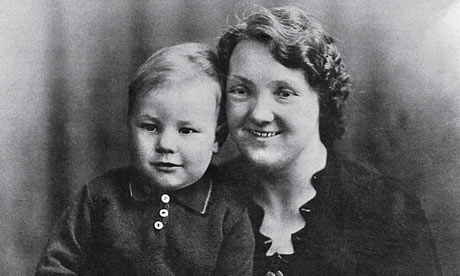
\includegraphics[width=0.3\textwidth]{kid.jpg}
  \end{center}
\end{frame}

\begin{frame}{Early Career}
  \begin{itemize}
    \item Dropped out of school at age 15 and got a job as a journalist
    \item Increased involvement in local theater
    \item After a year, quit journalism and decided to go to acting school
    \item Became a furniture salesman while saving money for Bristol Old Vic
    Acting School
  \end{itemize}
  \begin{fct}
    Sir Patrick Stewart lost his hair at age 19.
  \end{fct}
\end{frame}

\begin{frame}{Early Theatre Work}
  \begin{itemize}
    \item Joined the Manchester Library Theatre
    \item 1959 debut as Morgan in a stage adaptation of \emph{Treasure Island}
    \item Several brief appearances on British television (\emph{Coronation
    Street} and \emph{Civilisation})
    \item First major television appearance in 1974 as Lenin in \emph{Fall of
    Eagles}, and in \emph{I, Claudius} in 1976 as Sejanus
  \end{itemize}
\end{frame}

\begin{frame}{Shakespeare Influence}
  \begin{itemize}
    \item Member of Royal Shakespeare Company in 1966, Associate Artist with the Company in 1968
    \item Made Broadway debut in 1971 as Snout in \emph{A Midsummer's Night Dream}
    \begin{qct}
      \begin{quote}
        "We were, all of us, dazzled by the enthusiasm that the audience
        brought. Until the Macbeth, it was probably the biggest smash I had ever
        been in."
      \end{quote}
    \end{qct}
    \item Appeared in over 60 productions, most recently \emph{Hamlet} in 2008
  \end{itemize}
\end{frame}

\begin{frame}{Star Trek: The Next Generation}
  \begin{itemize}
    \item Starting in 1987, Stewart played the role of Jean-Luc Picard in the
    Science Fiction show Star Trek: TNG
    \item The show ran for seven years
    \item While the role at first did not seem to fit his Shakespearean roles he
    typically played, it became an obvious influence over the course of the show
    \item The science fiction role became an excellent way to provide an
    alternate view to the Shakespearean themes he typically portrayed.
  \end{itemize}
  \begin{qct}
    \begin{quote}
      "The fact is all of those years in Royal Shakespeare Company -- playing
      all those kings, emperors, princes and tragic heroes -- were nothing but
      preparation for sitting in the captain's chair of the Enterprise."
    \end{quote}
  \end{qct}
\end{frame}

\begin{frame}{Star Trek Movies}
  Stewart continued his role as Picard after the series in a number of
  motion pictures:
  \begin{itemize}
    \item \emph{Star Trek Generations}
    \item \emph{Star Trek: First Contact}
    \item \emph{Star Trek: Insurrection}
    \item \emph{Star Trek: Nemesis}
  \end{itemize}
  \begin{center}
    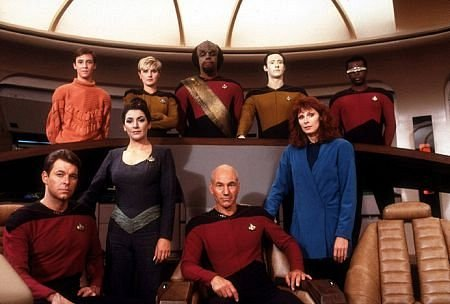
\includegraphics[width=0.6\textwidth]{tngcast.jpg}
  \end{center}
\end{frame}

\begin{frame}{X-Men}
  \begin{columns}
    \begin{column}{0.7\textwidth}
      \begin{itemize}
        \item Probably his most well known acting career, Stewart played the role of Professor
        Xavier in the X-Men series, including:
        \begin{itemize}
          \item{\emph{X-Men}}
          \item{\emph{X2}}
          \item{\emph{X-Men: The Last Stand}}
        \end{itemize}
        \item Also did voice acting for three X-Men based video games afterwards
        \item Developed a close friendship with Ian McKellen on the set
      \end{itemize}
    \end{column}
    \begin{column}{0.3\textwidth}
      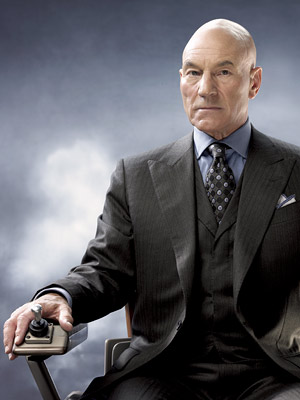
\includegraphics[width=0.8\textwidth]{xavier.jpg}
    \end{column}
  \end{columns}

\end{frame}

\begin{frame}{A Christmas Carol}
  \begin{columns}
    \begin{column}{0.7\textwidth}
      \begin{itemize}
        \item In 1991, Stewart performed an adaptation of Dicken's \emph{A Christmas
        Carol} where he acted over 40 different parts, effectively playing all
        the roles of the story himself.
        \item He produced the entire act, and even ran the company that produced
        it.
        \item Stewart received a Screen Actors Guild award nomination for the
        performance.
        \item He performed the act again in 1992, 1993, 1994, and 1996.
      \end{itemize}
    \end{column}
    \begin{column}{0.3\textwidth}
      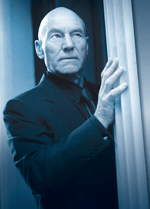
\includegraphics[width=0.8\textwidth]{xmascarol.png} \newline
      
\includegraphics[width=0.8\textwidth]{carol2.png} 
    \end{column}
  \end{columns}

\end{frame}

\begin{frame}{Other Films}
  \begin{itemize}
    \item 1984: Gurney Halleck in David Lynch's \emph{Dune}
    \item 1993: King Richard in \emph{Robin Hood: Men in Tights}
    \item 1999: Ebenezer Scrooge in \emph{A Christmas Carol}
    \item 2009: Vladimir in \emph{Waiting for Godot}
  \end{itemize}
\end{frame}

\begin{frame}{Voice Acting}
  \begin{columns}
    \begin{column}{0.7\textwidth}
      \begin{itemize} 
        \item 2005-2010: Avery Bullock on \emph{American Dad}
        \item 2007: Max Winters in \emph{TMNT}
        \item 2005: Lord Yupa in \emph{Nausicaa of the Valley of the Wind}
        \item 2001: \emph{Jimmy Neutron: Boy Genius} as King Goobot
        \item 1999: Napoleon in \emph{Animal Farm}
        \item 1995: The Simpsons!
        \item \emph{Star Trek} video games as Captain Picard
      \end{itemize}
    \end{column}
    \begin{column}{0.3\textwidth}
      
\includegraphics[width=0.9\textwidth]{Bullock.jpg} \newline
      
\includegraphics[width=0.9\textwidth]{HomertheGreat.png}
    \end{column}
  \end{columns}
\end{frame}

\begin{frame}{Personal Life}
  \begin{columns}
    \begin{column}{0.7\textwidth}
      \begin{itemize}
        \item Married to Sheila Falconer from 1966 to 1990, has a son and a daughter
        from that marriage
        \item Married to Wendy Neuss, a TNG producer, from 1997 to 2000
        \item Moved back to the UK from LA in 2004, after 17 years
        
      \end{itemize}
    \end{column}
    \begin{column}{0.3\textwidth}
      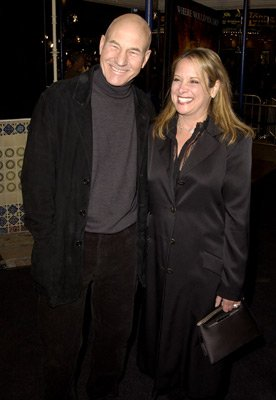
\includegraphics[width=0.8\textwidth]{withwife.jpg}
    \end{column}
  \end{columns}
  \begin{qct}
    \begin{quote}
      "From time to time, I have fantasies of becoming a concert
      pianist."
    \end{quote}
  \end{qct}
\end{frame}

\begin{frame}{Political Beliefs}
  Stewart's general beliefs can be summarized as fairness and equality.  
  \begin{itemize}
    \item Opposed the Iraq War
    \item Critized government for extending detention without charge to 42
    days, and signed a letter of objection to it.
    \item Advocates for legalization of assisted suicide
    \item Created a video for Amnesty International to help fight domestic
    violence, partly because of his memories of how his father treated his
    mother
    \item He is a member of the British Labour Party.
  \end{itemize}
  His childhood as a lower class citizen gave him perspective on social issues.

\end{frame}

\begin{frame}{Awards Received}
  \begin{itemize}
    \item 2010: Awarded Knighthood by Queen of England
    \item 2001: Awarded Officer of the Order of the British Empire
      \begin{qct}
        \begin{quote}
          "I'm very touched and very pleased with this and it was a delightful
          morning."
        \end{quote}
      \end{qct}
    \item 1992: Awarded "Sexiest Man on Television" by TV Guide
    \item 1991: Drama Desk Award for Outstanding One-Person for \emph{A
    Christmas Carol}
  \end{itemize}
\end{frame}

\begin{frame}{About this Presentation}
  This presentation was produced using only open-source software.

  The slides were created using Beamer and LaTeX.
  Group collaboration was done with git.
  \begin{center}
    
\includegraphics[width=0.6\textwidth]{engage.jpg}
  \end{center}
\end{frame}
\end{document}
